\PassOptionsToPackage{sols}{handout}
\documentclass[main]{subfiles}
\setcounterrefbeforedot{chapter}{m-ws6-6}
\setcounterrefafterdot{section}{m-ws6-6}
\addtocounter{section}{-1}
\usepackage{solutions}

\begin{document}

\ifSubfilesClassLoaded{%
  \chaptermark{\chaptersix}
}{}

\section{Area and Density Problems} \label{ws6-6}

\begin{problemonly}
    \begin{framed}

\textbf{Key Ideas}:

\begin{itemize}[topsep=0pt,partopsep=0pt,parsep=8pt,itemsep=0pt]


\item Area: 
  You should appreciate that there are times when a definite
  integral can be computed more easily by visualizing it as an area
  and slicing the areea horizontally rather than vertically.

\item Density: You should be comfortable with our strategy for     
  solving density problems:
  \begin{enumerate}[topsep=0pt,nosep]
  \item \textbf{Slice} the region so that the density in each slice is
    approximately constant.   (That is, within a single slice, the density
    does not vary much.) 
  \item \textbf{Approximate} the quantity you care about on each slice.
    (This should be easy since you can approximate the density within any
    given slice as being constant.) 
  \item \textbf{Sum these up} to get a Riemann sum approximation for what
    you're looking for.
  \item \textbf{Take the limit} as the number of slices $\to \infty$ to
    get a definite integral that gives you exactly what you're looking
    for! 
  \end{enumerate}

\item You should understand why we need to slice to solve density
  problems.  

\item You should be comfortable writing a Riemann sum that approximates
  the answer to a density problem, as well as the definite integral that
  gives the exact answer.


\end{itemize}
\end{framed}
\end{problemonly}

In the first two problems on this worksheet, we will look at how
a change in perspective can help us integrate some otherwise
challenging definite integrals. We will then adapt our newfound
flexibility to other situations in which it is necessary.

\begin{enumerate}

\item 
  \note{The point here is that, although $\displaystyle \int_1^e \ln x\,dx$
    is the obvious integral that expresses this area, it's an integral that needs to be evaluated by integration by parts. A more potentially more efficient way to evaluate this is to can slice the region
    horizontally to get an integral that we do know how to evaluate.}

  \begin{problem}[\vfill]
    Find the area under the curve $y = \ln x$ from $x = 1$ to $x = e$.
    (Please give your answer as a number, not an integral.)
  \end{problem}

  \begin{solution}
    Here is the area we are interested in:
    \begin{center}
      \begin{tikzpicture}
        \begin{axis}[axis on top=true, xmin=0, xtick={1, 2.718},
          xticklabels={1, $e$}, ytick={0, 1}, width=3in, height=2in,
          disabledatascaling] 
          \addplot+[domain=1:e, fillregion, draw=none] {1}
          \closedcycle; %
          \addplot+[fill=white, draw=none, domain=1:e] {ln(x)} -- (axis
          cs: 0, 2.718) -- (axis cs: 0, 0) -- (axis cs: 1, 0); %
          \addplot+[domain=0.8:3] {ln(x)}; %
          \draw (e, 0) -- (e, 1); %
        \end{axis}
      \end{tikzpicture}
    \end{center}
    We know that this area is $\displaystyle \int_1^e \ln x\,dx$, but
    we would need to use integration by parts to evaluate this integral. Since a goal is to develop flexibility in our integration, let's try another strategy.

    Let's \textbf{slice} the region into \textit{horizontal} strips of
    equal height $\Delta y$ (so we slice the interval $[0, 1]$ on the
    $y$-axis), label $y_0 = 0, \ldots, y_n = 1$ as usual, and focus on the
    $k$-th slice.
    \begin{center}
      \begin{tikzpicture}
        \begin{axis}[axis on top=true, xmin=0, xtick={1, 2.718},
          xticklabels={1, $e$}, ytick={0, 0.14286, ..., 1.01},
          yticklabels={$y_0 = 0$,,,,$y_k$,,, $y_n = 1$}, width=3in,
          height=2in, disabledatascaling, axis y line=left]
          \addplot+[domain=1:e, fillregion, draw=none] {1}
          \closedcycle; %
          \addplot+[fill=yellow, draw=none, domain=3/7:4/7] ({e^x}, x)
          -- (e, 4/7) -- (e, 3/7) -- cycle; %
          \addplot+[xcomb] coordinates { (e, 0) (e, 1/7) (e, 2/7) (e,
            3/7) (e, 4/7) (e, 5/7) (e, 6/7) (e, 1) }; %
          \addplot+[fill=white, draw=none, domain=1:e] {ln(x)} -- (axis
          cs: 0, 2.718) -- (axis cs: 0, 0) -- (axis cs: 1, 0); %
          \addplot+[domain=0.8:3] {ln(x)}; %
          \draw[dashed] (0, 4/7) -- ({e^(4/7)}, 4/7); %
          \draw (e, 0) -- (e, 1); %
        \end{axis}
      \end{tikzpicture}
    \end{center}
    The curve is $y = \ln x$, which we can also think of as $x = e^y$.
    We can \textbf{approximate} the slice by a rectangle (shown in
    blue):    
    \begin{center}
      \begin{tikzpicture}
        \begin{axis}[axis on top=true, xmin=0, xtick={1, 2.718},
          xticklabels={1, $e$}, ytick={0, 0.14286, ..., 1.01},
          yticklabels={$y_0 = 0$,,,,$y_k$,,, $y_n = 1$}, width=3in,
          height=2in, disabledatascaling, axis y line=left]
          \addplot+[domain=1:e, fillregion, draw=none] {1}
          \closedcycle; %
          \draw (e, 0) -- (e, 1); %
          \addplot+[fill=yellow, draw=none, domain=3/7:4/7] ({e^x}, x)
          -- (e, 4/7) -- (e, 3/7) -- cycle; %
          \addplot+[xcomb] coordinates { (e, 0) (e, 1/7) (e, 2/7) (e,
            3/7) (e, 4/7) (e, 5/7) (e, 6/7) (e, 1) }; %
          \addplot+[fill=white, draw=none, domain=1:e] {ln(x)} -- (axis
          cs: 0, 2.718) -- (axis cs: 0, 0) -- (axis cs: 1, 0); %
          \addplot+[domain=0.8:3] {ln(x)}; %
          \draw[dashed] (0, 4/7) -- ({e^(4/7)}, 4/7); %
          \draw[fill=cyan, draw=blue] ({e^(4/7)}, 4/7) -- (e, 4/7) --
          (e, 3/7) -- ({e^(4/7)}, 3/7) -- cycle; %
        \end{axis}
      \end{tikzpicture}      
    \end{center}
    Since the curve is $x = e^y$, the top left point of the rectangle has
    coordinates $\left( e^{y_k}, y_k \right)$.  The top right point has
    coordinates $(e, y_k)$.  Therefore, the width of the rectangle is $e -
    e^{y_k}$.  The rectangle has height $\Delta y$, so its area is $(e -
    e^{y_k}) \Delta y$.  So, we've shown that the area of the $k$-th slice
    is approximately $(e - e^{y_k}) \Delta y$.  \textbf{Summing} over all
    slices and \textbf{taking the limit} as the number of slices tends to
    infinity, we find that the area is $\displaystyle \lim_{n \to \infty}
    \sum_{k=1}^n (e - e^{y_k}) \Delta y$, which is equal to the integral
    $\displaystyle \int_0^1 (e - e^y)\,dy$.  We can easily evaluate this
    integral; it is equal to $\displaystyle ey - e^y \Big|_0^1 = (e - e) -
    (0 - 1) = \boxed{1}$.
  \end{solution}


\probonly{\newpage}

\item 
  \begin{problem}[\vfill]
    Let $\mathcal{R}$ be the region enclosed by $y = \arccos x$, the
    $x$-axis, and $x = - \frac{1}{2}$.  Find the area of $\mathcal{R}$.
    (Please evaluate your integral.)
  \end{problem}

  \begin{solution}
    Let's first sketch the region:
    \begin{center}
      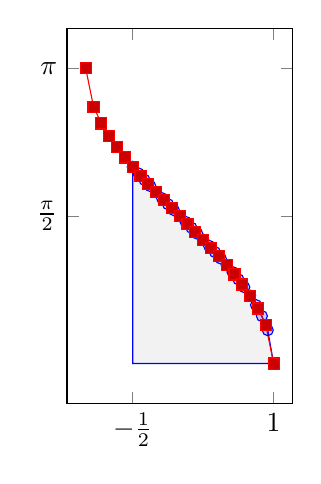
\begin{tikzpicture}
        \begin{axis}[xtick={-0.5, 1}, xticklabels={$-\frac{1}{2}$, $1$},
          ytick={1.57, 3.14}, yticklabels={$\frac{\pi}{2}$, $\pi$}, axis
          equal=true, width=1.75in, height=2.5in, enlarge x limits=true]
          \addplot+[domain=-0.5:1, fill=lightgray, fill opacity=0.2]
          {rad(acos(x))} \closedcycle; 
          \addplot+[domain=-1:1] {rad(acos(x))};
        \end{axis}
      \end{tikzpicture}
    \end{center}
    Although we can express the area as $\displaystyle \int_{-1/2}^1
    \arccos x\,dx$, that's not an integral that we know how to evaluate easily.
    So, let's instead slice horizontally, as we did in
    {{\#4}}.  First, notice that the top point of the
    region is $\left( - \frac{1}{2}, \arccos \left( - \frac{1}{2} \right)
    \right)$, or $\left( - \frac{1}{2}, \frac{2 \pi}{3} \right)$.  So,
    we'll slice the interval $\left[0, \frac{2 \pi}{3} \right]$ on the
    $y$-axis into $n$ slices of equal thickness $\Delta y$.  Labeling $y_0
    = 0, \ldots, y_n = \frac{2 \pi}{3}$ as usual, we can approximate the
    $k$-th slice as a rectangle: 
    \begin{center}
      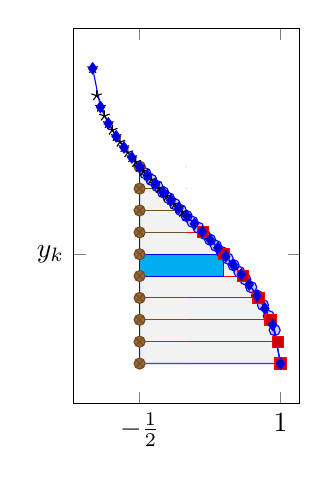
\begin{tikzpicture}[declare function={f(\x)=cos(deg(\x)); g(\x)=-1/2;}]
        \begin{axis}[xtick={-0.5, 1}, xticklabels={$-\frac{1}{2}$, $1$},
          ytick={1.16355}, yticklabels={$y_k$}, y tick label
          style={fill=none}, axis
          equal=true, width=1.75in, height=2.5in, enlarge x limits=true,
          disabledatascaling, axis on top=true] 
          \addplot+[domain=-0.5:1, fill=lightgray, fill opacity=0.2]
          {rad(acos(x))} \closedcycle; %
          \addplot+[xcomb] coordinates { ({f(0)}, 0) ({f(2*pi/27)},
            2*pi/27) ({f(4*pi/27)}, 4*pi/27) ({f(2*pi/9)}, 2*pi/9)
            ({f(8*pi/27)}, 8*pi/27) ({f(10*pi/27)}, 10*pi/27)
            ({f(4*pi/9)}, 4*pi/9) }; %
          \addplot+[xcomb] coordinates { ({g(0)}, 0) ({g(2*pi/27)},
            2*pi/27) ({g(4*pi/27)}, 4*pi/27) ({g(2*pi/9)}, 2*pi/9)
            ({g(8*pi/27)}, 8*pi/27) ({g(10*pi/27)}, 10*pi/27)
            ({g(4*pi/9)}, 4*pi/9) ({g(14*pi/27)}, 14*pi/27)
            ({g(16*pi/27)}, 16*pi/27) ({g(2*pi/3)}, 2*pi/3) }; %
          \addplot+[domain=-1:0, fill=white, draw=none] {rad(acos(x))} --
          (0, pi) -- (-1, pi); %
          \addplot+[domain=-1:1] {rad(acos(x))}; %
          \draw[fill=cyan, draw=blue] (-0.5, {10*pi/27}) -- 
          ({cos(deg(10*pi/27))}, {10*pi/27}) -- ({cos(deg(10*pi/27))},
          {8*pi/27}) -- (-0.5, {8*pi/27}) -- cycle; 
        \end{axis}
      \end{tikzpicture}
    \end{center}
    This rectangle has width (right $x$-coordinate) $-$ (left
    $x$-coordinate); the right side lies on the curve $y = \arccos x$ (or
    $x = \cos y$), and the left $x$-coordinate is $-\frac{1}{2}$.  The
    rectangle has height $\Delta y$, so
    \[ \text{area of $k$-th slice} \approx \left( \cos y_k - \left(-
        \frac{1}{2} \right) \right) \Delta y = \left( \cos y_k +
      \frac{1}{2} \right) \Delta y.\] Therefore, the area of the region is
    \begin{align*}
      \int_{0}^{2 \pi / 3} \left( \cos y + \frac{1}{2} \right)\,dy &=
      \left. \sin y + \frac{y}{2} \right|_0^{2 \pi / 3} \\
      &= \boxed{\frac{\sqrt{3}}{2} + \frac{\pi}{3}}
    \end{align*}
  \end{solution}


\probonly{\newpage}

\item 
  \note{This problem is just to get them thinking in the right direction:
    recognizing that the ``simple'' situation is when the density is
    constant.}

  \begin{problem}[0.5in]
    According to Wikipedia, the population density in Cambridge in the
    year 2000 was 15,000 people per square mile.  The area of Cambridge is
    about 7 square miles.  What was the population of Cambridge in the
    year 2000?
  \end{problem}

  \begin{solution}
    The population can be calculated easily:
    \begin{align*}
      \text{population} &= \text{(population density)} \cdot \text{(area
        of city)} \\ 
      & = (15,000 \text{ people per square mile}) \cdot
      (7 \text{ square miles}) \\
      & = \boxed{105,000 \text{ people}}
    \end{align*}
  \end{solution}

\item 
  A seaside village, Playa del Carmen, is in the shape of a rectangle with
  sides of 4 miles and 6 miles.  The sea lies along a 6-mile long side.
  People prefer to live near the water, so the density of people is given
  by $\rho(x) = 1000 (20 - x^2)$ people per square mile, where $x$ is the
  distance from the seaside.\probonly{\footnote{The symbol $\rho$ is the
      Greek letter ``rho'' and is pronounced ``row'' (as in ``Row, row,
      row your boat'').}}

  \begin{enumerate}
  \item 
    \note{This is intentionally somewhat vague, to get them to think about
      how we can approach this.  Ultimately, we want them to write a
      general Riemann sum (i.e., a Riemann sum with $n$ terms) to do this
      approximation.}  

    \begin{problem}[\vfill]
      How could you \textbf{approximate} the population of the
      village?
    \end{problem}

    \begin{solution}
      The key is to try to use the simple situation of
      {{\#3}}: if a region has a \textit{constant}
      population density, we can find the population simply by multiplying
      this density by the area of the region.

      Unfortunately, the village in this problem does not have a constant
      population density.  But since we are only trying to approximate the
      population, here is one strategy we could use:
      \begin{enumerate}[label=\arabic*.]
      \item \textbf{Slice} the village into pieces so that, within each
        piece, the density is pretty close to being constant (that is, the
        density doesn't vary too much).
      \item Then, we can \textbf{approximate} the population of a single
        piece by multiplying the approximately constant density of that
        piece by the area of the piece.
      \item That gives us an approximate population for one piece of the
        village; if we can do that for all pieces of the village, we can
        simply \textbf{sum} these approximations to get the approximate
        population of the entire village.
      \end{enumerate}
      Let's follow this strategy.  First, we'll draw a picture of the
      problem so that we can figure out how to slice.  The village is a
      rectangle, and let's draw it so that the 6-inch sides are vertical and
      the sea lies on the left.  (These are totally arbitrary choices.)
      Since $x$ represents distance from the sea, it is equal to 0 on the
      side of the village that touches the sea and equal to 4 on the
      opposite side.  The left picture below shows the village, the sea, and
      the meaning of $x$:
      \begin{center}
        
\includegraphics[height=1.5in]{images/density-rectangle-1}
        \hspace{0.5in}
        
\includegraphics[height=1.5in]{images/density-rectangle-1-density}
      \end{center}
      The right picture shows a way to visualize the density: by color.  For
      instance, when $x = 0$, the density is $\rho(0) = 20000$ people per
      square mile (colored red on the picture); when $x = 4$, the density is
      $\rho(4) = 4000$ people per square mile (colored in blue).  In
      general, as we get further from the sea, the density decreases.

      Now, let's go through our strategy in more detail: 
      \begin{itemize}
      \item \textbf{Step 1: Slice.}

        We want to slice the village into pieces so that, within each piece,
        the density is pretty close to being constant.  As we can see from
        our pictures, the way to achieve this is by slicing vertically.  If
        we look at a thin vertical slice of the village, the density does
        not vary much.  (In contrast, if we look at a thin horizontal slice
        of the village, the density still varies a lot, between 20000 and
        4000 people per square mile.)

        So, we'll slice the village into $n$ vertical strips of equal
        width $\Delta x$, and we'll label the $x$-values where we slice
        $x_0, x_1, \ldots, x_n$ as usual:
        \begin{center}
          
\includegraphics[height=1.5in]{images/density-rectangle-1-slices}
        \end{center}

      \item \textbf{Step 2: Approximate the population within a single
          slice.}

        We need to approximate the population in each slice, so let's look
        at the $k$-th slice: 
        \begin{center}
          
\includegraphics[height=1.5in]{images/density-rectangle-1-kth-slice}
        \end{center}
        We can approximate the
        population in the $k$-th slice as
        \begin{align*}
          \text{population in $k$-th slice} & \approx (\text{population
            density in $k$-th slice}) \cdot (\text{area of $k$-th slice})
          \\
          \intertext{Since the population density does not vary much within
            a slice, we can approximate the population density in the
            $k$-th slice as $\rho(x_k)$.  The slice is shaped like a
            rectangle of width $\Delta x$ and height $6$, so its area is
            $6 \Delta x$:}
          & \approx \rho(x_k) \cdot 6 \Delta x
        \end{align*}

      \item \textbf{Step 3: Sum.}

        We figured out that the population in the $k$-th slice is
        approximately $\rho(x_k) \cdot 6 \Delta x$.  So, for instance, the
        population in the first slice ($k = 1$) is approximately $\rho(x_1)
        \cdot 6 \Delta x$, the population in the second slice ($k = 2$) is
        approximately $\rho(x_2) \cdot 6 \Delta x$, and so on.  To
        approximate the population of the whole village, we just add up the
        populations of all the slices.  This gives
        \[ \boxed{\rho(x_1) \cdot 6 \Delta x + \rho(x_2) \cdot 6 \Delta x
          + \cdots + \rho(x_n) \cdot 6 \Delta x}\] as our approximation
        for the population of the village.  In sigma notation, this is
        $\boxed{\sum_{k=1}^n \rho(x_k) \cdot 6 \Delta x}$.  
      \end{itemize}
    \end{solution}

  \item
    \begin{problem}[0.75in]
      What is the \textbf{exact} population of the village?
    \end{problem}

    \begin{solution}
      Taking the limit as $n \to \infty$ of our Riemann sum $\displaystyle
      \sum_{k=1}^n \rho(x_k) \cdot 6 \Delta x$, the exact population of
      the village is
      \begin{align*}
        \boxed{\int_0^4 \rho(x) \cdot 6\,dx} &= 6000 \int_0^4 (20 -
        x^2)\,dx \\
        &= 6000 \left( \left. 20 x - \frac{x^3}{3} \right|_0^4 \right) \\
        &= 6000 \left( 80 - \frac{64}{3} \right) \\
        &= \boxed{352,000 \text{ people}}
      \end{align*}
    \end{solution}

  \end{enumerate}

\end{enumerate}

\end{document}